\begin{figure}[H]
	\center
	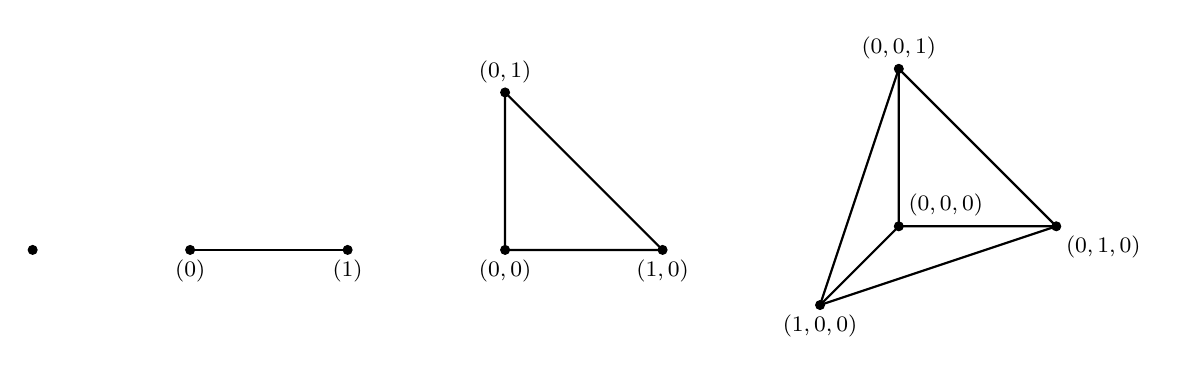
\begin{tikzpicture}[scale=2]
	\filldraw (0,0) circle (0.8pt);
	%      \fill[black,font=\footnotesize] (0,0) node[below] {$(0)$};
	
	\draw[thick] (1,0) -- ++(1,0);
	\filldraw (1,0) circle (0.8pt);
	\filldraw (1,0) ++(1,0) circle (0.8pt);
	\fill[black,font=\footnotesize] (1,0) node[below] {$(0)$}
									(1,0) ++(1,0) node[below] {$(1)$};
	
	\draw[thick] (3,0) -- ++(0,1) -- ++(1,-1)--cycle;
	\filldraw (3,0)         circle (0.8pt);
	\filldraw (3,0) ++(1,0) circle (0.8pt);
	\filldraw (3,0) ++(0,1) circle (0.8pt);
	\fill[black,font=\footnotesize] (3,0)         node[below] {$(0,0)$}
									(3,0) ++(0,1) node[above] {$(0,1)$}
									(3,0) ++(1,0) node[below] {$(1,0)$};
	
	\draw[thick] (5.5,0.15) -- ++(0,1) --++(1,-1) -- cycle;
	\draw[thick] (5.5,0.15)  -- ++(-0.5,-0.5); -- ++(1.5,0.5);
	\draw[thick] (5.5,0.15) ++(0,1) -- ++(-0.5,-1.5) -- ++(1.5,0.5);
	\filldraw (5.5,0.15) circle (0.8pt);
	\filldraw (5.5,0.15) ++(0,1) circle (0.8pt);
	\filldraw (5.5,0.15) ++(1,0) circle (0.8pt);
	\filldraw (5.5,0.15) ++(-0.5,-0.5) circle (0.8pt);
	\fill[black,font=\footnotesize] (5.5,0.15) node[above right] {$(0,0,0)$}
									(5.5,0.15) ++(0,1) node[above] {$(0,0,1)$}
									(5.5,0.15) ++(1,0) node[below right] {$(0,1,0)$}
									(5.5,0.15) ++(-0.5,-0.5) node[below] {$(1,0,0)$};
	
	%\node at (3.2,-0.9) {unity simplex  for $d=0,\dots,3$};
	\end{tikzpicture}
		
	\caption{unity simplex $\hat{\tau}$ for $d=0,\dots,3$}
	\label{ch1_unity_simplex}

\end{figure}